\section{Reverse-Correlation Methods: Simple Cells}
\label{sec:ReverseCorrelationMethodsForSimpleCells}
\begin{defn}
  \label{def: spikeTriggeredAverage}
  Given the light intensity of a visual image $s(s,y,t)$ and a spike sequence $\{t_i\}_{i = 1}^n$, the \emph{spike-triggered average stimulus}  is a function of three variables
  \begin{equation}
    \label{equ:2.21}
    C(x,y,\tau) = \frac{1}{\left<n\right>}\left<\sum\limits_{i = 1}^ns(x,y,t_i-\tau)\right>,
  \end{equation}
  where the brackets denote trial averaging, and we have used the approximation $1/n \approx 1/\left<n\right>$.
\end{defn}

\begin{defn}
  \label{def:crrelationFuncForVisual}
  The \emph{correlation function} between the firing rate at time $t$ and the stimulus at time $t+\tau$, for trials of duration $T$ is defined as
  \begin{equation}
    \label{equ:2.22}
    Q_{rs}(x,y,\tau) = \frac{1}{T}\int_0^Tr(t) s(x,y,t+\tau)dt.
  \end{equation}
\end{defn}

\begin{prop}
  \label{prop:CQ_relation}
  The spike-triggered average is related to the reverse-correlation function by
  \begin{equation}
    \label{equ:2.23}
    C(x,y,\tau) = \frac{Q_{rs}(x,y,-\tau)}{\left<r\right>},
  \end{equation}
  where $\left<r\right> = \left<n\right>/T$ is as usual, the average firing rate over the entire trial.
\end{prop}
\begin{proof}
  The proof is similar with the one in Chapter \ref{cha:Neural Encoding I}.
\end{proof}

\begin{rem}
  To estimate the firing rate of a neuron in response to a particular image, we add a function of the output of a linear filter of the stimulus to the background firing rate $r_0$, as in Equation \ref{equ:2.8}, $r_{\rm{est}}(t) = r_0 + F(L(t))$. Because visual stimuli depend on spatial location, we must decide how contributions from different image locations are to be combined to determine $L(t)$. Note that, firing rates are not a function of $x$ and $y$.
\end{rem}

\begin{defn}
  \label{def:linearResponseEstimate}
  Suppose that the contributions from linear response estimate different spatial points sum linearly, the \emph{linear response estimate} $L(t)$ is obtained by integrating over all $x$ and $y$ values:
  \begin{equation}
    \label{equ:2.24}
    L(t) = \int_0^{\infty}\iint D(s,y,\tau)s(x,y,t-\tau)dxdyd\tau,
  \end{equation}
  where the kernel $D(x,y,\tau)$ determines how strongly, and with what sign, the visual stimulus at the point $(x,y)$ and at time $t-\tau$ affects the firing rate of the neuron at time $t$.
\end{defn}

\begin{prop}
  The optimal kernel is given in terms of the firing rate-stimulus correlation function, or the spike-triggered average, for a white-noise stimulus with variance parameter $\sigma_s^2$ by
  \begin{equation}
    \label{equ:2.25}
    D(x,y,\tau) = \frac{Q_{rs}(x,y,-\tau)}{\sigma_s^2} = \frac{\left<r\right>C(x,y,\tau)}{\sigma_s^2}.
  \end{equation}
\end{prop}
\begin{proof}
  The proof is similar with the one in Chapter \ref{cha:Neural Encoding I}.
\end{proof}

\begin{defn}
  \label{def:space-timeReceptiveField}
  The kernel $D(x,y,\tau)$ defines the \emph{space-time receptive field} of a neuron.
\end{defn}

\begin{rem}
  Because $D(x,y,\tau)$ is a function of three variables, it can be difficult to measure and visualize.
\end{rem}

\begin{defn}
  \label{def:separableReceptiveField}
  If the spatial structure of one neuron's receptive field does not change over time except by an overall multiplicative factor, the kernel can be written as a product of two functions, one that describes the \emph{spatial receptive field} and the other, the \emph{temporal receptive field},
  \begin{equation}
    \label{equ:2.26}
    D(x,y,\tau) = D_s(x,y)D_t(\tau).
  \end{equation}
  Such neurons are said to have \emph{separable space-time receptive field}.
\end{defn}

\begin{defn}
  \label{def:nonseparableReceptiveField}
  When $D(x,y,\tau)$ cannot be written as the product of two terms, the neuron is said to have a \emph{nonseparable space-time receptive field}.
\end{defn}

\begin{asm}[Normalization]
  \label{asm:Normalized}
  Given the freedom in Equation \ref{equ:2.8} to set the scale of $D$ (by suitably adjusting the function $F$), we typically normalize $D_s$ so that its integral is $1$, and use a similar rule for the components from which $D_t$ is constructed, that is,
  \begin{displaymath}
    \iint D_s(x,y)dxdy = 1 \ \rm{and} \ \int_0^{\infty}D_t(\tau)d\tau = 1.
  \end{displaymath}
\end{asm}

\begin{rem}
  We begin our analysis by studying first the spatial and then the temporal components of a separable space-time receptive field, and then proceed to the nonseparable case. For simplicity, we ignore the possibility that cells can have slightly different receptive fields for the two eyes, which underlies the disparity tuning considered in chapter \ref{cha:Neural Encoding I}.
\end{rem}

\subsection{Spatial Receptive Fields}
\label{sec:SpatialReceptiveFields}

\begin{defn}
  \label{def:regions}
  Regions within the receptive field where $D_s$ is positive, is called \emph{ON regions}, and where it is negative, is called \emph{OFF regions}.
\end{defn}

\begin{exm}
  \label{exm:spatialExm}
  The following figures show the spatial structure of the receptive fields of two neurons in cat primary visual cortex determined by averaging stimuli between 50 ms and 100 ms prior to an action potential, that is, $\int_{50}^{100}C(x,y,\tau)d\tau/50$.
  \begin{center}
    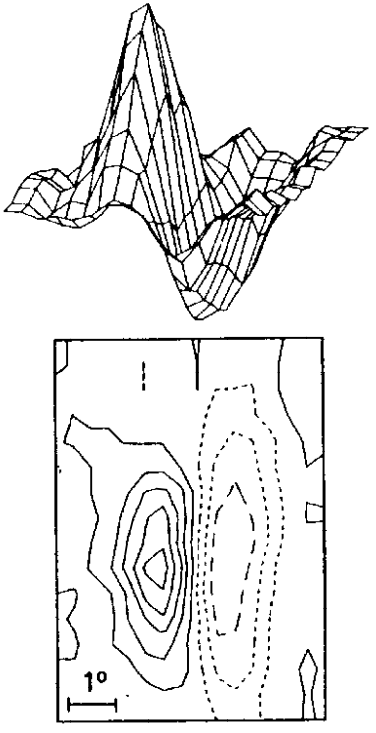
\includegraphics[scale=0.2]{./png/spatialExm1}
    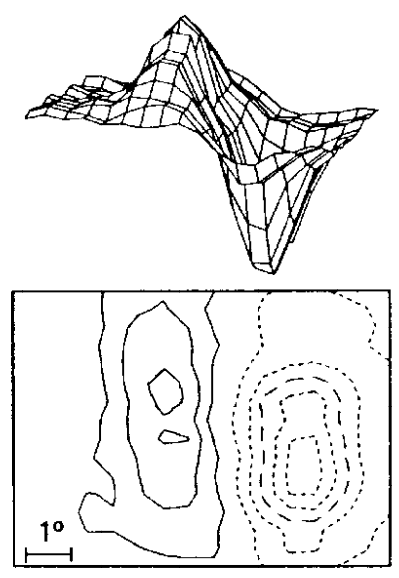
\includegraphics[scale=0.25]{./png/spatialExm2}
  \end{center}
  The upper plots are three-dimensional representations, with the horizontal dimensions acting as the $x$-$y$ plane and the vertical dimension indicating the magnitude and sign of $D_s(x, y)$. The lower contour plots represent the $x$-$y$ plane. Regions with solid contour curves are ON areas where $D_s(x, y) > 0$, and regions with dashed contours are OFF areas where $D_s(x, y) < 0$.
\end{exm}

\begin{prop}
  \label{prop:OnOffEffect}
  The response of a neuron is enhanced if ON regions are illuminated ($s>0$) or if OFF regions are darkened ($s<0$) relative to the background level of illumination. Conversely, they are suppressed by darkening ON regions or illuminating OFF regions.
\end{prop}
\begin{proof}
  The integral of the linear kernel times the stimulus can be visualized by noting how the OFF and ON regions overlap the image.
\end{proof}

\begin{rem}
  From Proposition \ref{prop:OnOffEffect}, the neurons of figures in Example \ref{exm:spatialExm} respond most vigorously to light-dark edges positioned along the border between the ON and OFF regions, and oriented parallel to this border and to the elongated direction of the receptive fields, shown below.
\end{rem}

\begin{exm}
  \label{exm:spatialStimuliExm}
  Grating stimuli superimposed on spatial receptive fields similar to those shown in Example \ref{exm:spatialExm}.  The receptive field is shown as two oval regions, one dark to represent an OFF area where $D_s<0$ and one white to denote an ON region
where $D_s>0$.
  \begin{center}
    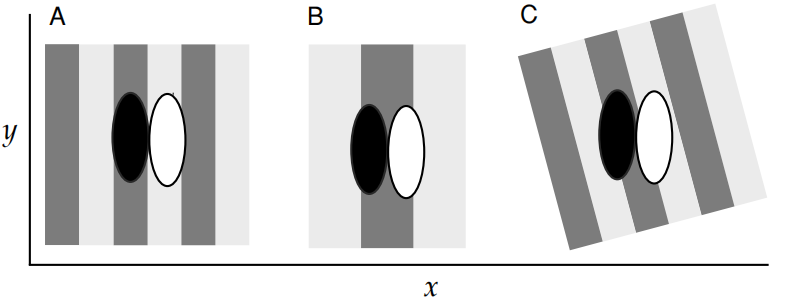
\includegraphics[scale=0.3]{./png/spatial_stimuliExm}
  \end{center}
\end{exm}

\begin{rem}
  The above examples show receptive fields with two major subregions. Simple cells are found with from one to five subregions. Along with the ON-OFF patterns we have seen, another typical arrangement is a three-lobed receptive field with OFF-ON-OFF or ON-OFF-ON subregions.
\end{rem}

\begin{defn}
  \label{def:GaborFunc}
  A \emph{Gabor function} is a product of a Gaussian function and a sinusoidal function.
\end{defn}

\begin{defn}
  If the coordinates $x$ and $y$ are chosen such that the borders between the ON and OFF regions are parallel to the $y$ axis and the origin of the coordinates is placed at the center of the receptive field, the Gabor function
  \begin{equation}
    \label{equ:2.27}
    D_s(x,y) = \frac{1}{2\pi\sigma_x\sigma_y}\exp\left(-\frac{x^2}{2\sigma_x^2}-\frac{y^2}{2\sigma_y^2}\right)\cos(kx-\phi)
  \end{equation}
  can be used to approximate the observed receptive field structures.
  The parameters in this function determine the properties of the spatial receptive field:
  \begin{enumerate}[(i)]
  \item $\sigma_x$ and $\sigma_y$, the \emph{receptive field size}, determine its extent in the $x$ and $y$ directions, respectively.
  \item $k$, the \emph{preferred spatial frequency}, determines the spacing of light and dark bars that produce the maximum response (the preferred spatial wavelength is $2\pi/k$).
  \item $\phi$, the \emph{preferred spatial phase}, determines where the ON-OFF boundaries fall within the receptive field.
  \end{enumerate}
\end{defn}

\begin{prop}
  For the spatial receptive field Equation \ref{equ:2.27}, the sinusoidal grating described by Equation \ref{equ:2.18} that produces the maximum response for a fixed value of $A$ has $K = k$, $\Phi = \phi$, and $\Theta = 0$.
\end{prop}

\begin{ntn}%%think more
  The Gabor functions mentioned below refer to Equation \ref{equ:2.27}.
\end{ntn}

\begin{exm}
  The Gabor functions chosen specifically to match the data in Example \ref{exm:spatialExm}. These two figures are plotted with $\sigma_x = 1^{\circ}$, $\sigma_y = 2^{\circ}$, $1/k = 0.56^{\circ}$ and $\phi = 1 - \pi/2$ (left), $\phi = 1 - \pi$ (right).
  \begin{center}
    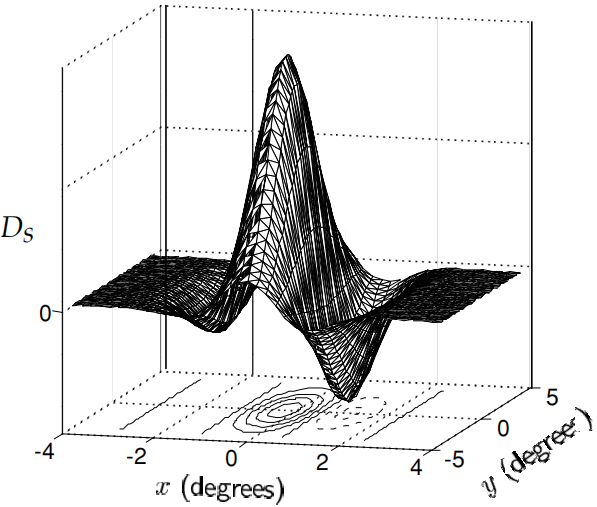
\includegraphics[scale=0.2]{./png/Gabor1}
    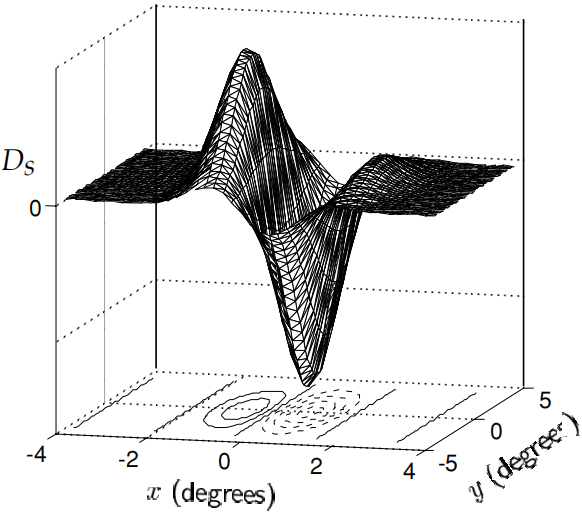
\includegraphics[scale=0.2]{./png/Gabor2}
  \end{center}
\end{exm}

\begin{exm}
  \label{exm:SplitGabor}
  $x$- and $y$- plots of a variety of Gabor functions (Equation \ref{equ:2.27}) with different parameter values. For convenience, these plots are the dimensionless function $2\pi\sigma_x\sigma_yD_s$.
  \begin{center}
    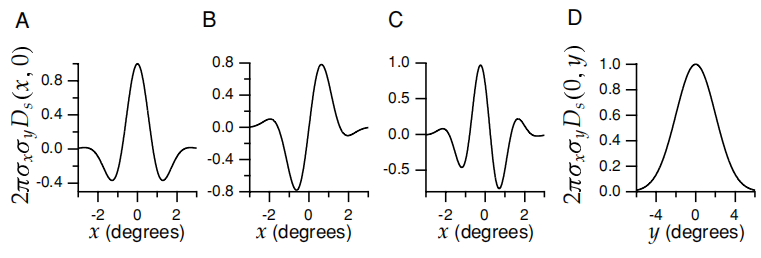
\includegraphics[scale=0.33]{./png/GaborSplitExm}
  \end{center}
  Responding parameters are as follows:
  \begin{enumerate}[(i)]
  \item A with $\sigma_x = 1^{\circ}$, $1/k = 0.5^{\circ}$, $\phi = 0$ and $y = 0$ is symmetric about $x = 0$.
  \item B with $\sigma_x = 1^{\circ}$, $1/k = 0.5^{\circ}$, $\phi = \pi/2$ and $y = 0$ is antisymmetric about $x = 0$ and corresponds to using a sine instead of a cosine function in Equation \ref{equ:2.27}.
  \item C with $\sigma_x = 1^{\circ}$, $1/k = 0.33^{\circ}$, $\phi = \pi/4$ and $y = 0$ has no particular symmetry properties with respect to $x = 0$.
  \item D with $\sigma_y = 2^{\circ}$ and $x = 0$ is simply a Gaussian.
  \end{enumerate}
\end{exm}

\begin{rem}
  As seen in Example \ref{exm:SplitGabor}, Gabor functions can have various types of symmetry, and variable numbers of significant oscillations (or subregions) within the Gaussian envelope.
\end{rem}

\begin{rem}
  The response characterized by Equation \ref{equ:2.27} is maximal if light-dark edges are parallel to the $y$ axis, so the preferred orientation orientation for a stimulus is 0.
\end{rem}

\begin{prop}
  An arbitrary preferred orientation $\theta$ can be generated by rotating the coordinates, making the substitutions $x \to a\cos(\theta)+y\sin(\theta)$ and $y \to y\cos(\theta)-x\sin(\theta)$ in Equation \ref{equ:2.27}. This produces a spatial receptive field that is maximally responsive to a grating with $\Theta = \theta$.
\end{prop}
\begin{proof}
  Actually, this rotation is from the rotation matrix
  \begin{displaymath}
    M(\theta) = \left(
      \begin{matrix}
        \cos(\theta) & \sin(\theta)\\
        -\sin(\theta) & \cos(\theta)
      \end{matrix}
    \right),
  \end{displaymath}
  which rotates a vector in two-dimensional space by $\theta$ clockwise.
\end{proof}

\begin{prop}
  Similarly, a receptive field centered at the point $(x_0, y_0)$ rather than at the origin can be constructed by making the substitutions $x \to x-x_0$ and $y \to y-y_0$, where the $(x_0, y_0)$ is called the \emph{receptive field center}.
\end{prop}

\subsection{Temporal Receptive Fields}
\label{sec:TemporalReceptiveFields}

\begin{exm}
  \label{exm:TimeDevelopExm}
  The following figure reveals the temporal development of the space-time receptive field of a neuron in the cat primary visual cortex through a series of snapshots of its spatial receptive field.
  Each panel is a plot of $D(x, y,\tau)$ for a different value of $\tau$. The curves below the contour diagrams are one-dimensional plots of the receptive field as a function of $x$ alone. Around $\tau$ = 210 ms, a two-lobed OFF-ON receptive field is evident. As $\tau$ decreases, this structure first fades away and then reverses, so that the receptive field at $\tau$ = 75 ms has the opposite sign from what appeared at $\tau$ = 210 ms.
  \begin{center}
    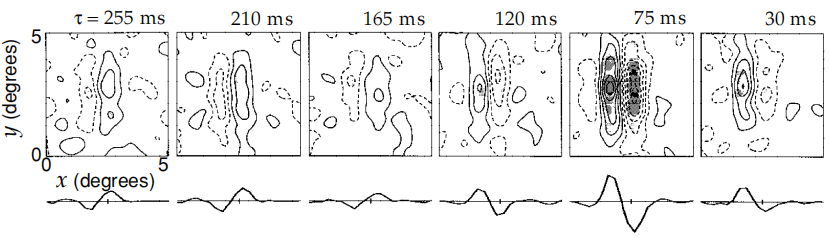
\includegraphics[scale=0.3]{./png/timeDevelopExm}
  \end{center}
  The stimulus preferred by this cell is thus an appropriately aligned
dark-light boundary that reverses to a light-dark boundary over time.
\end{exm}

\begin{rem}
  In the above figure, for $\tau >$ 300 ms, there is little correlation between the visual stimulus and the upcoming spike. Due to latency effects, the spatial structure of the receptive field is less significant for $\tau <$ 75 ms.
\end{rem}

\begin{prop}
   The neuron in Example \ref{exm:TimeDevelopExm} has approximately a separable space-time receptive field.
\end{prop}
\begin{proof}
  Although the magnitudes and signs of the different spatial regions vary over time, their locations and shapes remain fairly constant. This indicates that the neuron has, to a good approximation, a separable space-time receptive field.
\end{proof}

\begin{defn}
  The phenomenon that a neuron's receptive field reverses with time is called the \emph{reversal effect}.
\end{defn}

\begin{rem}
  Reversal effects are a common feature of space-time receptive fields.
\end{rem}

\begin{prop}
  \label{prop:twoPhaseReact}
  The reversal can be described by a function
  \begin{equation}
    \label{equ:2.29}
    D_t(\tau) = \left\{
      \begin{array}{ll}
        \alpha \exp(-\alpha\tau)\left(\frac{(\alpha\tau)^5}{5!} - \frac{(\alpha\tau)^7}{7!}\right) & \tau \geq 0,\\
        0 & \tau < 0.\\
      \end{array} \right.
  \end{equation}
  Here, $\alpha$ is a constant that sets the scale for the temporal development of the function.
\end{prop}
\begin{proof}
  The function $D_t(\tau)$ of Equation \ref{equ:2.29} rises from 0, becomes positive, then negative, and ultimately returns to 0 as $\tau$ increases.
\end{proof}

\begin{exm}
  Temporal structure of a receptive field. (Plot $D_t(\tau)$ in Equation \ref{equ:2.29} with $\alpha$ = 1/(15 ms).)
  \begin{center}
    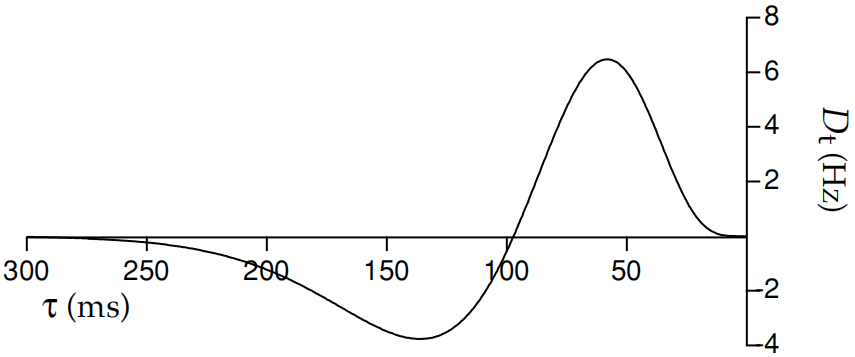
\includegraphics[scale=0.25]{./png/temporalReceptiveField}
  \end{center}
\end{exm}

\begin{rem}
  Single-phase responses are also seen for V1 neurons, and these can be described by eliminating the second term in Equation \ref{equ:2.29}. Three-phase responses, which are sometimes seen, must be described by a more complicated function.
\end{rem}

\subsection{Response of a Simple Cell to a Counterphase Grating}
\label{sec:ResponseOfSimpleCelltoCounterphaseGrating}

\begin{rem}
  The response of a simple cell to a counterphase grating stimulus (Equation \ref{equ:2.18}) can be estimated by computing the function $L(t)$.
\end{rem}

\begin{prop}
  For the separable receptive field, the linear estimate of the response can be written as the product of two terms,
  \begin{equation}
    \label{equ:2.30}
    L(t) = L_sL_t(t),
  \end{equation}
  where
  \begin{equation}
    \label{equ:2.31}
    L_s = \iint D_s(x,y)A\cos\left( Kx\cos(\Theta)+Ky\sin(\Theta)-\Phi\right) dxdy
  \end{equation}
  and
  \begin{equation}
    \label{equ:2.32}
    L_t(t) = \int_0^{\infty}D_t(\tau)\cos(\omega(t-\tau))d\tau.
  \end{equation}
\end{prop}

\begin{asm}
  We assume that $D_s(x,y)$ and $D_t(\tau)$ used in this section are from Equation \ref{equ:2.27} and \ref{equ:2.29}, respectively.
\end{asm}

\begin{exc}
  Compute these integrals in equations \ref{equ:2.31} and \ref{equ:2.32} for $D_s(x,y)$ in Equation \ref{equ:2.27} with $\sigma_x = \sigma_y = \sigma$ and $D_t(\tau)$ in Equation \ref{equ:2.29}.
\end{exc}

\begin{prop}
  If the spatial phase of the stimulus and the preferred spatial phase of the receptive field are 0 ($\Phi = \phi = 0$),
  \begin{equation}
    \label{equ:2.33}
    L_s = A\exp\left(-\frac{\sigma^2(k^2+K^2)}{2}\cosh(\sigma^2kK\cos(\Theta))\right),
  \end{equation}
  which determines the orientation and spatial frequency tuning for an
optimal spatial phase.
\end{prop}

\begin{lem}
  \label{lem:anApproximation}
  For a grating with the preferred orientation $\Theta = 0$ and a spatial frequency that is not too small, the full expression for $L_s$ can be simplified by noting that $\exp(-\sigma^2kK) \approx 0$ for the values of $k\sigma$ noemally encountered.
\end{lem}

\begin{exm}
  If $K = k$ and $k\sigma = 2$, $\exp(-\sigma^2kK) = 0.02$.
\end{exm}

\begin{prop}
  Using the approximation in Lemma \ref{lem:anApproximation},
  \begin{equation}
    \label{equ:2.34}
    L_s = \frac{A}{2}\exp\left(-\frac{\sigma^2(k-K)^2}{2}\right)\cos(\phi-\Phi),
  \end{equation}
  which reveals a Gaussian dependence on spatial frequency and a cosine
dependence on spatial phase.
\end{prop}

\begin{exm}
  Selectivity of a Gabor filter (Equation \ref{equ:2.31} with $D_s(x,y)$ from Equation \ref{equ:2.27}) with $\theta = \phi = 0$, $\sigma_x = \sigma_y = \sigma$, and $k\sigma = 2$ acting on a cosine grating with $A = 1$.
  \begin{center}
    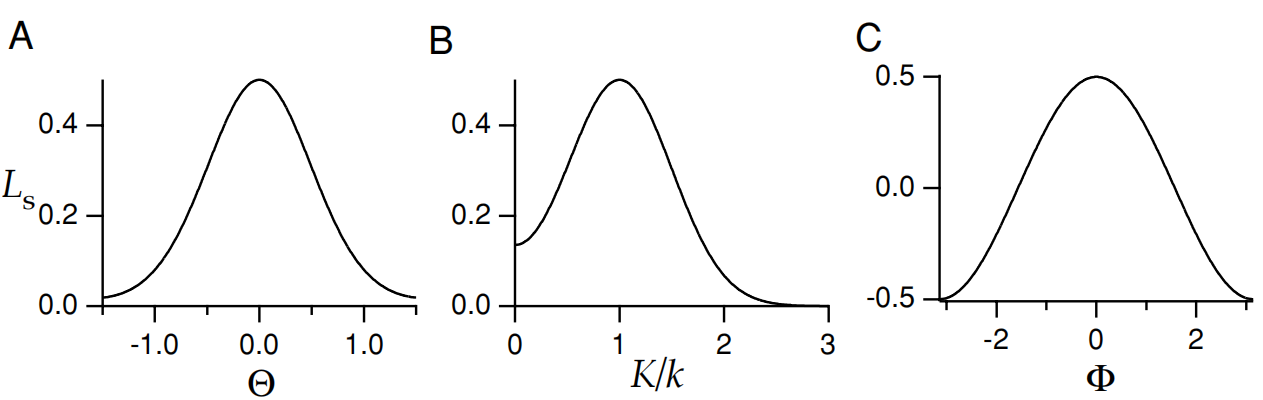
\includegraphics[scale=0.2]{./png/showSelectivity}
  \end{center}
  (A) $L_s$ as a function of stimulus orientation $\Theta$ for a grating with the preferred spatial frequency and phase, $K = k$ and $\Phi = 0$. (B) $L_s$ as a function of the ratio of the stimulus spatial frequency to its preferred value, $K/k$, for a grating oriented in the preferred direction $\Theta = 0$ and with the preferred phase $\Phi = 0$. (C) $L_s$ as a function of stimulus spatial phase $\Phi$ for a grating with the preferred spatial frequency and orientation, $K = k$ and $\Theta = 0$.
\end{exm}

\begin{exm}
  % Frequency response of a model simple cell based on the temporal kernel of Equation \ref{equ:2.29}. The amplitude of the sinusoidal oscillations of $L_t(t)$ produced by a counterphase grating is plotted as a function of the temporal oscillation frequency, $\omega/2\pi$ rather than the angular frequency $\omega$.
  The temporal frequency dependence of the amplitude of the linear response estimate  is plotted as a function of the temporal frequency of the stimulus ($\omega/2\pi$ rather than the angular frequency $\omega$).
  \begin{center}
    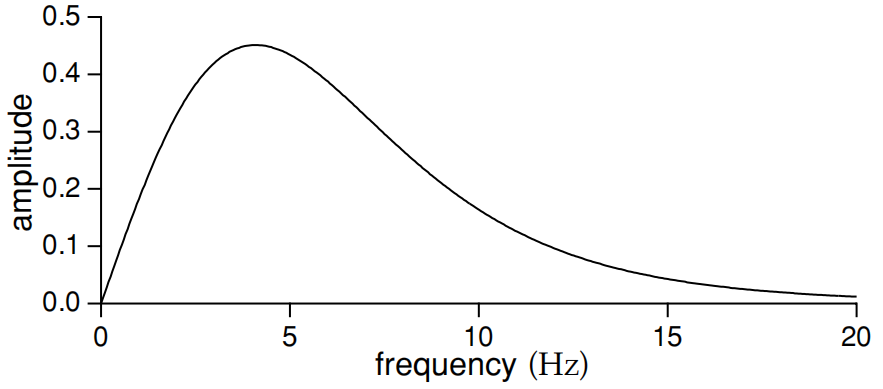
\includegraphics[scale=0.25]{./png/frequencyAmplitude}
  \end{center}
  The peak value around 4 Hz and roll-off above 10 Hz are typical for V1 neurons and for cortical neurons in other primary sensory areas as well.
\end{exm}

\subsection{Space-Time Receptive Fields}
\label{sec:Space-TimeReceptiveFields}

\begin{rem}
  To display the function $D(x, y,\tau)$ in a space-time plot rather than as a sequence of spatial plots , we suppress the $y$ dependence and plot an $x$-$\tau$ projection of the space-time kernel.
\end{rem}

\begin{exm}[ A separable space-time receptive field]
  \label{exm:separableSpaceTimePlotExm}
  Figure A shows a space-time plot of the receptive field of a simple cell in the cat primary visual cortex. This receptive field is approximately separable, and it has side-by-side OFF and ON regions that reverse as a function of $\tau$.
  \begin{center}
    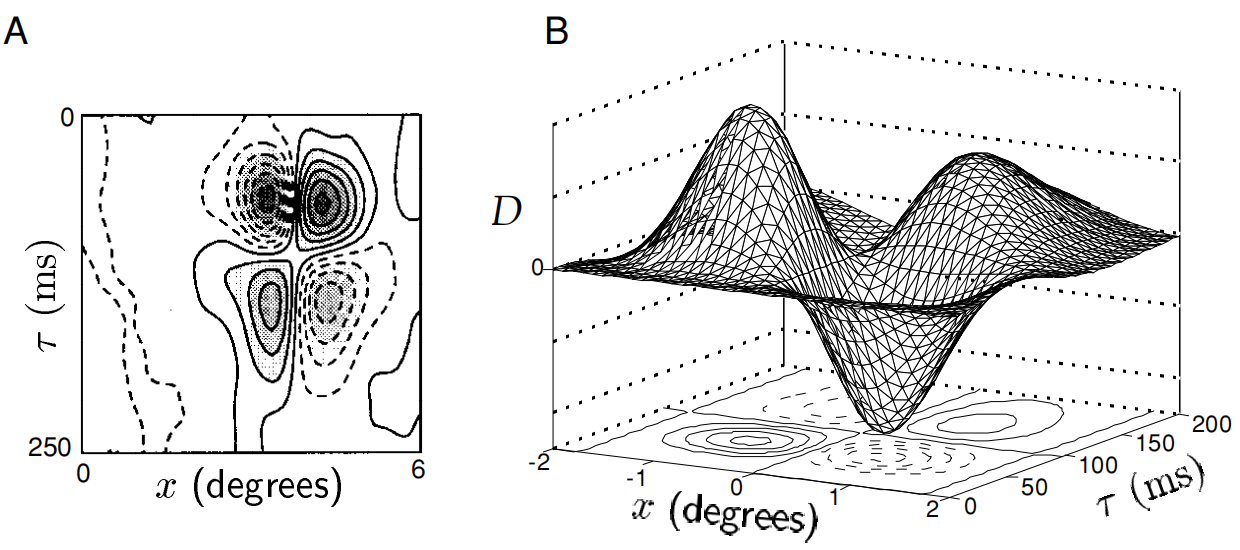
\includegraphics[scale=0.2]{./png/spaceTimePlotExm}
  \end{center}
  Figure B shows an $x$-$\tau$ plot of a separable space-time kernel, similar to the one in A, generated by multiplying a Gabor function (evaluated at $y = 0$) with $\sigma_x = 1^{\circ}$, $1/k = 0.56^{\circ}$ and $\phi = \pi/2$ by the temporal kernel of Equation \ref{equ:2.29} with $1/\alpha = 15$ ms.
\end{exm}

\begin{rem}
  We can also plot the visual stimulus in a space-time diagram, suppressing the $y$ coordinate by assuming that the image does not vary as a function of $y$.
\end{rem}

\begin{exm}[Space and space-time diagrams of a moving grating]
  Figure A shows a grating of vertically oriented stripes moving to the left on an $x$-$y$ plot. In the $x$-$t$ plot of figure B, this image appears as a series of sloped dark and light bands. These represent the
projection of the image in A onto the $x$ axis evolving as a function of time. The leftward slope of the bands corresponds to the leftward
movement of the image.
  \begin{center}
    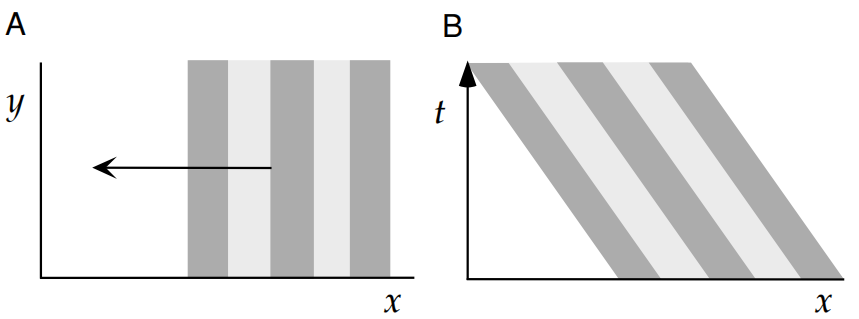
\includegraphics[scale=0.3]{./png/spaceTimeDiagramExm1}
  \end{center}
\end{exm}

\begin{prin}
  \label{prin:responseSelectivity}
  Most neurons in primary visual cortex do not respond strongly to static images, but respond vigorously to flashed and moving bars and gratings.
\end{prin}

\begin{rem}
  The receptive field structure of Example \ref{exm:separableSpaceTimePlotExm} reveals why this is the case in Principle \ref{prin:responseSelectivity}.
\end{rem}

\begin{exm}[Why a flashed bar is a effective stimulus]
  \label{exm:explain1}
  The following figures show responses to dark bars estimated from a separable space-time receptive field.
  \begin{center}
    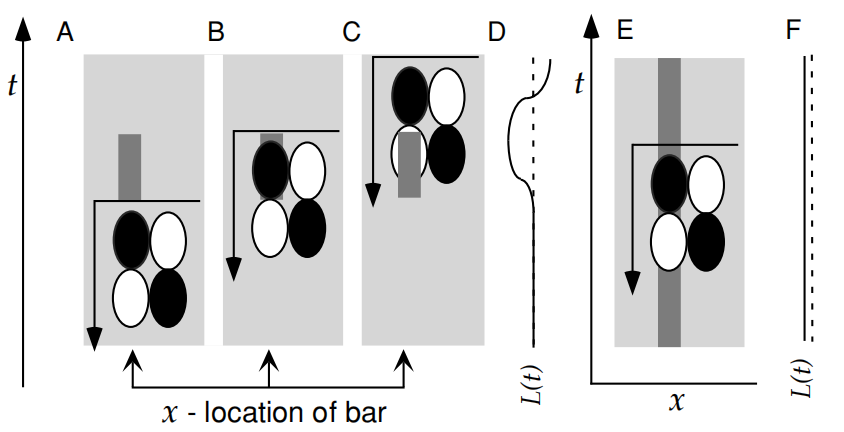
\includegraphics[scale=0.27]{./png/responseSelectivityExplain1}
  \end{center}
  The linear estimate of the response at any time is determined by positioning the receptive field diagram so that its horizontal axis matches the time of response estimation and noting how the OFF and ON regions overlap with the image.
  \begin{enumerate}[]
  \item (A-C) The image is a dark bar that is flashed on for a short interval of time. There is no response (figure A) until the dark image overlaps the OFF region (figure B) when $L(t)>0$. The response is later suppressed when the dark bar overlaps the ON region (figure C) and $L(t) < 0$.
  \item  (D) A plot of $L(t)$ versus time corresponding to the responses generated in figures A-C. Time runs vertically in this plot, and $L(t)$ is plotted horizontally with the dashed line indicating the zero axis and positive values plotted to the left.
  \item (E) The image is a static dark bar. The bar overlaps both an OFF (small $\tau$) and an ON (large $\tau$) region, generating opposing positive and negative contributions to $L(t)$.
  \item (F) The weak response corresponding to E, plotted as in figure D.
  \end{enumerate}
  The flashed dark bar of figures A-C is a more effective stimulus than the static bar of figure E.
\end{exm}

\begin{exm}[Why a moving grating is a particularly effective stimulus]
  \label{exm:explain2}
  The following figure shows responses to moving gratings estimated from a separable space-time receptive field. The receptive field is the same as in Example \ref{exm:explain1}.
  \begin{center}
    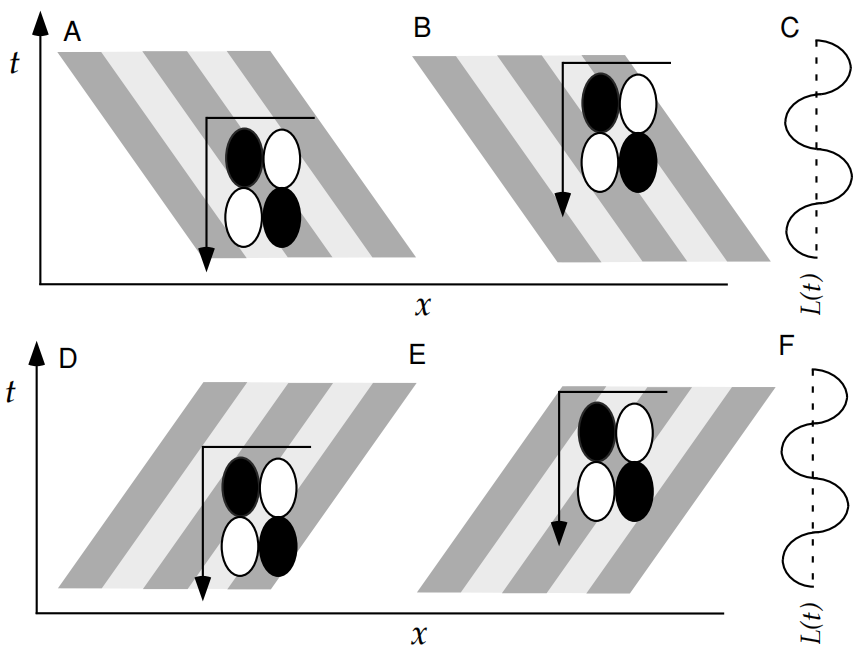
\includegraphics[scale=0.27]{./png/responseSelectivityExplain2}
  \end{center}
  \begin{enumerate}[]
  \item (A-C) The stimulus is a grating moving to the left.
    \begin{enumerate}[-]
    \item At the time corresponding to figure A, OFF regions overlap with dark bands and ON regions with light bands, generating a strong response.
    \item At the time of the estimate in figure B, the alignment is reversed, and $L(t)$ is negative.
    \item Figure C is a plot of $L(t)$ versus time corresponding to the responses generated in figures A-B. Time runs vertically in this plot and $L(t)$ is plotted horizontally, with the dashed line indicating the zero axis and positive values plotted to the left.
    \end{enumerate}
  \item (D-F) The stimulus is a grating moving to the right. The responses are identical to those in figures A-C.
  \end{enumerate}
\end{exm}

\begin{rem}
   Separable space-time receptive fields can produce responses that are maximal for certain speeds of grating motion, but they are not sensitive to the direction of motion.
 \end{rem}

 \subsection{Nonseparable Receptive Fields}
\label{sec:NonseparableReceptiveFields}

\begin{rem}
  Many neurons in primary visual cortex are selective for the direction of motion of an image. Accounting for direction selectivity requires nonseparable space-time receptive fields.
\end{rem}

\begin{exm}
  \label{exm:nonseparableReceptiveFieldExm}
  An example of a nonseparable receptive field is shown as below. This neuron has a three-lobed OFF-ON-OFF spatial receptive field, and these subregions shift to the left as time moves forward (and $\tau$ decreases). This means that the optimal stimulus for this neuron has light and dark areas that move toward the left.
  \begin{center}
    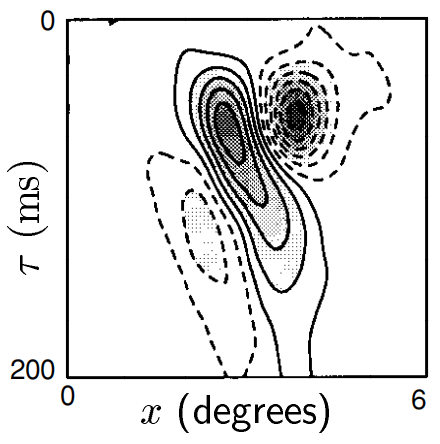
\includegraphics[scale=0.3]{./png/nonseparableReceptiveFieldExm}
  \end{center}
\end{exm}

\begin{rem}
  One way to describe a nonseparable receptive field structure is to use a separable function constructed from a product of a Gabor function for $D_s$ and Equation \ref{equ:2.29} for $D_t$, but to write these as functions of a mixture or rotation of the $x$ and $\tau$ variables.
\end{rem}

\begin{lem}
  \label{lem:rotarionMatrix}
  The rotation matrix
  \begin{equation}
    \label{equ:rotationMatrix}
    M'(\psi) = \left(
      \begin{matrix}
        \cos(\psi) & -\sin(\psi) \\
        \sin(\psi) & \cos(\psi) \\
      \end{matrix}
    \right)
  \end{equation}
  can rotates a vector in two-dimensional space by $\psi$ counterclockwise.
\end{lem}

\begin{prop}
  The rotation of the space-time receptive field is achieved by mixing the space and time coordinates, using the transformation
  \begin{equation}
    \label{equ:2.35}
    D(x,y,\tau) = D_s(x',y)D_t(\tau')
  \end{equation}
  with
  \begin{equation}
    \label{equ:2.36}
    x' = x\cos(\psi) - c\tau\sin(\psi)
  \end{equation}
  and
  \begin{equation}
    \label{equ:2.37}
    \tau' = \tau\sin(\psi) + \frac{x}{c}\sin(\psi),
  \end{equation}
  where factor $c$ converts between the units of time (ms) and space (degrees), and $\psi$ is the space-time rotation angle.
\end{prop}
\begin{proof}
  Note that the origin of $x$-$\tau$ plot in Example \ref{exm:nonseparableReceptiveFieldExm} is on the upper left corner, thus this rotation should be counterclockwise. Equation \ref{equ:2.36} and \ref{equ:2.37} follow from Lemma \ref{lem:rotarionMatrix} directly.
\end{proof}

\begin{exm}
  \label{exm:nonseparableReceptiveFieldEst1}
  Mathematical description of the space-time receptive field in Example \ref{exm:nonseparableReceptiveFieldExm} constructed from equations \ref{equ:2.35} - \ref{equ:2.37}. The parameters are selected as follows:
  \begin{enumerate}[(i)]
  \item The Gabor function used (evaluated at $y = 0$) had $\sigma_x = 1^{\circ}$, $1/k = 0.5^{\circ}$, and $\phi = 0$.
  \item $D_t$ is given by the expression in Equation \ref{equ:2.29} with $\alpha = 20$ ms, except that the second term, with the seventh power function, was omitted because the receptive field does not reverse sign in this example.
  \item The $x$-$\tau$ rotation angle used was $\psi = \pi/9$, and the conversion factor was $c = 0.02^{\circ}$/ms.
  \end{enumerate}
  \begin{center}
    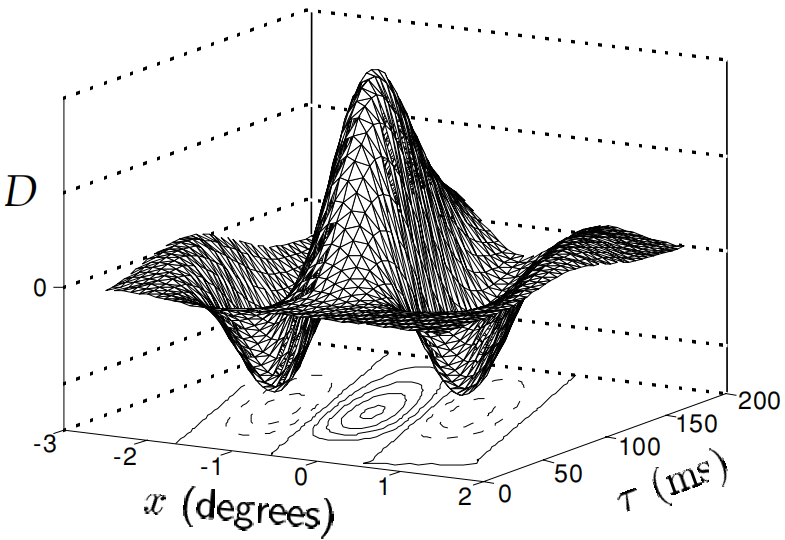
\includegraphics[scale=0.25]{./png/nonseparableReceptiveFieldEst1}
  \end{center}
\end{exm}

\begin{rem}
  The rotation operation is not the only way to generate nonseparable space-time receptive fields. They are often constructed by adding together two or more separable space-time receptive fields with different spatial and temporal characteristics.
\end{rem}

\begin{exm}[Direction Sensitivity]
  \label{exm:directionSensitivity}
  The following figures show responses to moving gratings estimated from a nonseparable spacetime receptive field.
  \begin{center}
    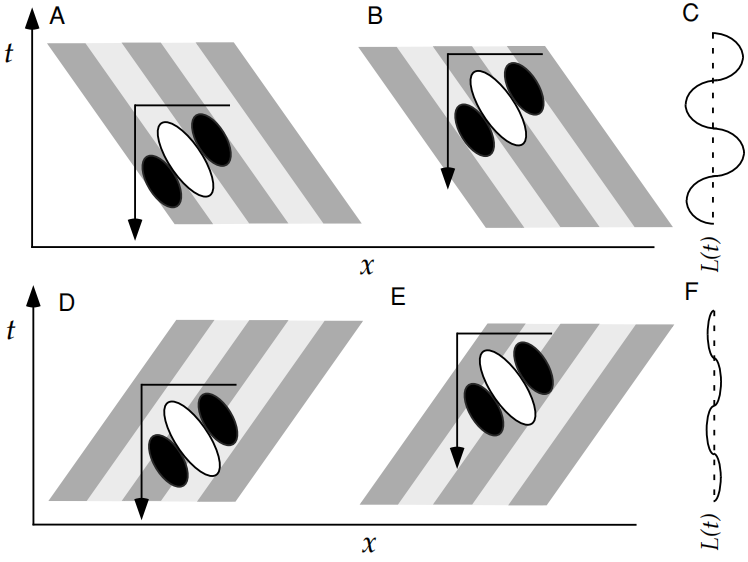
\includegraphics[scale=0.3]{./png/directionSensitivity}
  \end{center}
  \begin{enumerate}[]
  \item (A-C) The stimulus is a grating moving to the left.
    \begin{enumerate}[-]
    \item At the time corresponding to figure A, OFF regions overlap with dark bands and the ON region overlaps a light band, generating a strong response.
    \item At the time of the estimate in figure B, the alignment is reversed, and $L(t)$ is negative.
    \item Figure C is a plot of $L(t)$ versus time corresponding to the responses generated in figures A-B.
    \end{enumerate}
  \item (D-F) The stimulus is a grating moving to the right. Because of the tilt of the space-time receptive field, the alignment with the right-moving grating is never optimal and the response is weak (figure F).
  \end{enumerate}
\end{exm}

\begin{rem}
  Although $x$-corrdination of the receptive field in the Example \ref{exm:directionSensitivity} changes over time, the variation range of $x$ is only the range displayed by the three oval regions. $x$ does not always move in one direction over time, but move periodically within this range over time.
\end{rem}

\begin{rem}
  As a result, a neuron with a nonseparable space-time receptive field can be \emph{selective for the direction of motion} of a grating and \emph{for its velocity}, responding most vigorously to an optimally spaced grating moving at a velocity given by $c\tan(\psi)$. That is, the moving velocity of the space-time receptive field is the \emph{preferred velocity}.
\end{rem}

\subsection{Static Nonlinearities: Simple Cells}
\label{sec:StaticNonlinearitiesForSimpleCells}

\begin{rem}
  Once the linear response estimate $L(t)$ has been computed, the firing rate of a visually responsive neuron can be approximated by using Equation \ref{equ:2.8}, $r_{\rm{est}}(t) = r_0 +F(L(t))$, where $F$ is an  appropriately chosen static nonlinearity.
\end{rem}

\begin{exm}
  \label{exm:simpleF}
  The simplest choice for F consistent with the positive nature of firing rates is rectification, $F = G[L]_+$, with $G$ set to fit the magnitude of the measured firing rates.
\end{exm}

\begin{rem}
  However, the choice in Example \ref{exm:simpleF} makes the firing rate a linear function of the contrast amplitude, which does not match the data on the contrast dependence of visual responses.
\end{rem}

\begin{defn}
  \label{defn:contrastSaturation}
  The \emph{contrast saturation} means neural responses saturate as the contrast of the image increases, and are more accurately described contrast saturation by
  \begin{displaymath}
    r \propto A^n/(A_{1/2}^n + A^n)
  \end{displaymath}
  where $n$ is near 2, and $A_{1/2}$ is a parameter equal to the contrast amplitude that produces a half-maximal response.
\end{defn}

\begin{prop}
  A static nonlinearity defined by
  \begin{equation}
    \label{equ:2.38}
    F(L) = \frac{G[L]_+^2}{A_{1/2}+G[L]_+^2}
  \end{equation}
  reproduces the observed contrast dependence.
\end{prop}



%%% Local Variables:
%%% mode: latex
%%% TeX-master: "../notesOnFluidMechanics"
%%% End:
